\section{Method}
\label{sec:method}
\begin{figure*}[h] 
    \centering  
    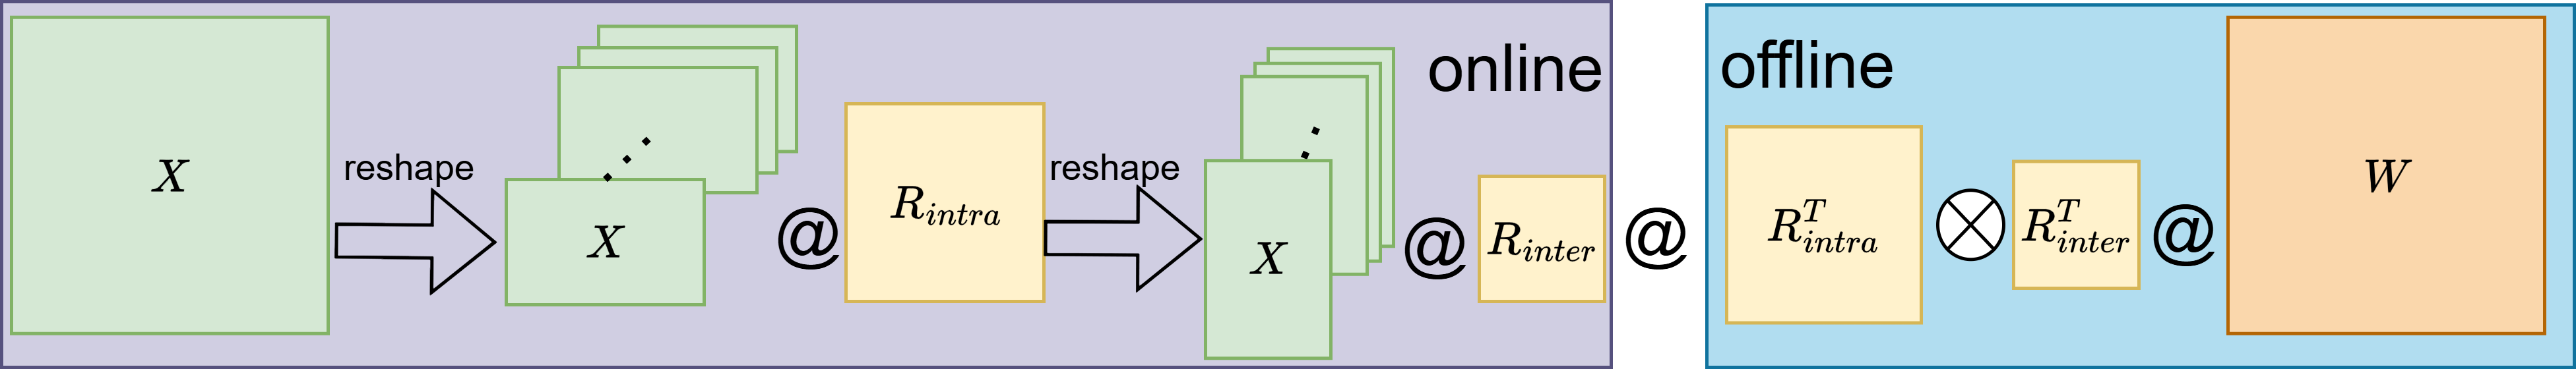
\includegraphics[width=0.95\textwidth]{img/fig-fram.png}
    \caption{TORQ algorithm's complete process framework.}
    \label{fig:fram}
\end{figure*}
% \vspace{-3mm}

Our objective is to find an orthogonal transformation $\mathbf{R} \in \mathcal{O}(d)$ such that the quantization error of the rotated activations $\mathbf{Z} = \mathbf{X}\mathbf{R}$ in the MXFP4 format is minimized:
\begin{equation}
\min_{\mathbf{R} \in \mathcal{O}(d)} \mathbb{E} \left[ \| \mathbf{X}\mathbf{R} - Q_{\text{mxFP4}}(\mathbf{X}\mathbf{R}) \|_F^2 \right]
\end{equation}
Directly optimizing a high-dimensional orthogonal matrix $\mathbf{R}$ is computationally intractable and difficult to converge. To address this, TORQ decomposes $\mathbf{R}$ into two structured sub-transformations: Inter-block rotation $\mathbf{R}_{\text{inter}}$ and Intra-block rotation $\mathbf{R}_{\text{intra}}$, such that $\mathbf{R} = \mathbf{R}_{\text{inter}} \otimes \mathbf{R}_{\text{intra}}$. This decomposition not only reduces optimization complexity but, more importantly, achieves decoupled control over "energy" and "distribution." During the inference phase, the overhead of the inverse transformation can be nearly eliminated by fusing it with the weights of the adjacent linear layer. If the quantized activation $\hat{\mathbf{z}}$ is input to a linear layer $\mathbf{W} \in \mathbb{R}^{d' \times d}$ (where $d = B K$), the fused weight becomes $\mathbf{W}' = \mathbf{W} (\mathbf{R}_{\text{intra}}^\top \otimes \mathbf{R}_{\text{inter}}^\top)$, where $\otimes$ denotes the Kronecker product. Figure.\ref{fig:fram} illustrates the overall framework.

\subsection{Macro-Equilibrium Rotation: Inter-block Rotation based on the Schur-Horn Theorem}

The core objective of inter-block rotation is to achieve global equilibrium of variances across all blocks at the same position via orthogonal transformation, thereby eliminating the dominance of a few high-variance blocks over the total error. The design is based on rigorous convex optimization theory and an efficient engineering construction method.

\subsubsection{Theoretical Foundation: Optimality under Convex Error Models}

For the reshaped activation matrix with structure $B \times K$, assuming the expected mean within blocks is 0, we define the block variance vector $\boldsymbol{\sigma}^2 \in \mathbb{R}^B$, where $\sigma_b^2 = \|\mathbf{z}_b\|_2^2$.

\begin{theorem}[Optimality of Variance Equalization]
\label{thm:optimality}
Assuming the quantization MSE $\phi_b(\sigma^2)$ of block $b$ is a convex function of its input variance $\sigma^2$, the total MSE satisfies:
\begin{equation}
\min_{\mathbf{R}^{(k)} \in \mathcal{O}(B)} \sum_{b=1}^B \phi_b\left([\mathbf{R}^{(k)}\boldsymbol{\Sigma}_k\mathbf{R}^{(k)\top}]_{bb}\right) = \sum_{b=1}^B \phi_b\left(\frac{\mathrm{tr}(\boldsymbol{\Sigma}_k)}{B}\right)
\end{equation}
Equality holds if and only if $\mathrm{diag}(\mathbf{R}^{(k)}\boldsymbol{\Sigma}_k\mathbf{R}^{(k)\top}) = \frac{\mathrm{tr}(\boldsymbol{\Sigma}_k)}{B}\mathbf{1}$ (i.e., all block variances are equal), where $\mathcal{O}(B)$ denotes the group of orthogonal matrices of order $B$, and $\mathbf{1}$ is the all-ones vector.
\end{theorem}

\textit{Proof Sketch.} The Schur-Horn theorem~\cite{schur_horn} states that there exists an orthogonal matrix $\mathbf{R}^{(k)}$ such that the diagonal elements of the transformed covariance matrix can be any vector majorized by the eigenvalues. Under convex functions and constraints, the uniform allocation (constant vector) minimizes the objective function. The complete proof is provided in Appendix A.1.
% The convexity assumption of the error function forms the theoretical basis of Theorem 4.1. In practical engineering, even if the above convexity assumption does not hold, variance smoothing, derived from its outlier suppression mechanism, can still act as an effective "soft limiter" by redistributing the energy of high-variance blocks to low-variance blocks: it reduces the upper limit of the block sharing index ($s_b$), thereby mitigating the quantization noise caused by aggressive scaling.
Beyond the theoretical bounds established by convexity, the practical utility of variance equalization lies in suppressing local maxima. By redistributing energy from high-variance to low-variance blocks, TORQ acts as a dynamic 'soft clipper' that reduces the peak magnitudes determining the shared exponents ($s_b$)2. This effectively lowers the scaling factor ceiling, mitigating the severe resolution loss caused by outliers.

% \begin{lemma}[Convexity of MXFP4 Error Model]
% The block MSE $\phi_b(\sigma^2)$ of MXFP4 block floating-point quantization satisfies convexity. The block MSE of MXFP4 is determined by quantization granularity error, distribution shape factors, and codeword matching factors. Its core term $\exp(2\cdot\mathrm{Var}(\log_2|\mathbf{a}_b|))$ is monotonically increasing and has a non-negative second derivative with respect to block variance $\sigma^2$. Therefore, $\phi_b(\sigma^2)$ is a convex function, satisfying the conditions of Theorem \ref{thm:optimality}. We further demonstrate the convexity of the MXFP4 error model in Appendix A.2.
% \end{lemma}

% \textbf{Key Corollary:} In the context of MXFP4 quantization, a rotation configuration that achieves perfectly balanced inter-block variance is the global optimal solution for minimizing total MSE. This theoretically validates the rationale behind inter-block rotation.

Proposition 4.2 (Empirical Error Behavior). While the strict convexity of the block MSE holds under high-rate quantization assumptions \cite{zamir}, in the coarse 4-bit regime, the error is dominated by the scaling factor $s_b$.

Analysis: The block-wise shared exponent $s
_b$ is determined by the maximum magnitude in the block. Outliers inflate $s_b$, increasing the quantization step size $\sigma=s_b \dot \sigma_{base}$
for all elements. By reducing the variance disparity between blocks (Theorem 4.1), TORQ effectively lowers the expectation of the maximum values, thereby minimizing the average scaling factor and reducing the global quantization noise. Although theoretical convexity is an approximation for discrete FP4, our extensive experiments confirm that variance equalization acts as an effective proxy for MSE minimization.

\subsubsection{Efficient Construction of Orthogonal Matrices: Schur-Horn Driven Givens Rotation}

Based on Theorem \ref{thm:optimality}, we need to construct an orthogonal matrix $\mathbf{R}_{\text{inter}}$ for all position $k$ such that $\mathrm{diag}(\mathbf{R}_{\text{inter}}\boldsymbol{\Sigma}_k\mathbf{R}^\top_{\text{inter}}) = c\mathbf{1}$, where $c=\mathrm{tr}(\boldsymbol{\Sigma}_k)/B$. We design an efficient iterative Givens rotation algorithm (Algorithm \ref{alg:givens}) that ensures convergence within $\mathcal{O}(B^2)$ time.

\begin{algorithm}[tb]
   \caption{Givens Rotation for Variance Equalization}
   \label{alg:givens}
\begin{algorithmic}[1]
   \STATE {\bfseries Input:} Covariance matrix $\boldsymbol{\Sigma} \in \mathbb{R}^{B \times B}$, convergence threshold $\epsilon$
   \STATE {\bfseries Output:} Orthogonal matrix $\mathbf{R} \in \mathcal{O}(B)$ such that $\mathrm{diag}(\mathbf{R}\boldsymbol{\Sigma}\mathbf{R}^\top) \approx c\mathbf{1}$
   \STATE Initialize $\mathbf{R} = \mathbf{I}_B$, calculate target $c = \mathrm{tr}(\boldsymbol{\Sigma})/B$
   \WHILE{$\max_i |\sigma_{ii} - c| > \epsilon$}
       \STATE Select block pair $(i, j)$ with opposite variance deviation signs, i.e., $(\sigma_{ii} - c)(\sigma_{jj} - c) < 0$
       \STATE Calculate rotation angle $\theta = \frac{1}{2}\arctan \frac{2\sigma_{ij}}{\sigma_{ii} - \sigma_{jj}}$
       \STATE Construct Givens rotation matrix $\mathbf{G}_{ij}(\theta)$
       \STATE Update $\boldsymbol{\Sigma} \leftarrow \mathbf{G}^\top \boldsymbol{\Sigma} \mathbf{G}$, $\mathbf{R} \leftarrow \mathbf{R}\mathbf{G}$
   \ENDWHILE
   \STATE {\bfseries return} $\mathbf{R}$
\end{algorithmic}
\end{algorithm}
% \vspace{-6mm}

\subsection{Micro-Alignment Rotation: Intra-block Rotation based on Codebook Alignment}

The goal of intra-block rotation is to reshape the intra-block activation distribution via orthogonal transformation in the normalized MXFP4 codeword space, ensuring that activation values uniformly occupy all available codewords, thereby maximizing the effective utilization of the 4-bit floating-point codebook.

\subsubsection{Computational Graph and Normalized FP4 Space}

Consider the activation matrix $\mathbf{X} \in \mathbb{R}^{B \times K}$ after inter-block rotation. We insert an identity transformation link into the computational graph:
\begin{equation}
\mathbf{X} \xrightarrow[]{\mathbf{S}^{-1}} \mathbf{X}_{\text{norm}} \xrightarrow[]{\mathbf{R}_{\text{intra}}} \mathbf{Z} \xrightarrow[]{Q_{\text{mxFP4}}} \hat{\mathbf{Z}} \xrightarrow[]{\mathbf{R}_{\text{intra}}^\top \mathbf{S}} \hat{\mathbf{X}}
\end{equation}
where $\mathbf{S} = \mathrm{diag}(s_1, \dots, s_B) \in \mathbb{R}^{B \times B}$ is the block-wise scaling matrix with shared scale $s_b$ for each block $b$, and $\mathbf{R}_{\text{intra}} \in \mathbb{R}^{K \times K}$ is the intra-block orthogonal rotation matrix. Under full precision, this link is strictly equivalent to an identity mapping. $\mathbf{S}^{-1}$ normalizes each block to the natural scale of MXFP4 (Normalized FP4 Space), and $\mathbf{R}_{\text{intra}}$ rearranges the statistical distribution of columns within this space.

\subsubsection{Codebook Occupancy Equilibrium Loss}

Let the set of positive codewords for MXFP4 (e2m1) be $\{c_1, \dots, c_J\}$ (where $J=8$), corresponding to decision boundaries $\{d_0=0, d_1, \dots, d_J=+\infty\}$. We define the \textbf{Codebook Occupancy Equilibrium Loss} as:
\begin{equation}
\mathcal{L}_{\text{code}}(\mathbf{S}, \mathbf{R}_{\text{intra}}) = \sum_{j=1}^{J} \left( \hat{p}_j(\mathbf{S}, \mathbf{R}_{\text{intra}}) - \frac{1}{J} \right)^2
\end{equation}
where $\hat{p}_j$ is the empirical codeword occupancy probability. This loss directly quantifies the "imbalance" of MXFP4 codeword usage, aligning precisely with the logarithmic geometric structure of MXFP4.
% 【Discussion on Non-uniformity: We acknowledge that the MXFP4 format is non-uniform, with larger quantization steps in high-value regions (e.g., gap is 2.0 for value 4-6 vs 0.5 for 0-2). Strictly speaking, a uniform histogram (Max Entropy) might push more data into high-error regions compared to an ideal MSE-minimal distribution.
% However, in the context of activation quantization, the dominant failure mode is Codebook Collapse—where most data falls into the zero bin. The gain from "activating" these idle codewords (via Max Entropy) orders of magnitude outweighs the precision loss from the non-uniform grid. TORQ serves as a first-order correction to ensure codebook utilization.】

\subsubsection{Alternating Optimization Framework: S-step and R-step}

We employ an alternating coordinate descent strategy to iteratively optimize $\mathbf{S}$ and $\mathbf{R}_{\text{intra}}$.

\textbf{S-step (Update Block Scaling):} Fix $\mathbf{R}_{\text{intra}}$, and for each block $b$, map its maximum activation value to the maximum MXFP4 codeword $c_{\max}$:
\begin{equation}
s_b \leftarrow \text{clip\_to\_pow2}\left( \frac{\max_i |z_{b,i}|}{c_{\max}} \right)
\end{equation}

\textbf{R-step (Update Intra-block Rotation):} Fix $\mathbf{S}$ and update $\mathbf{R}_{\text{intra}}$ through a series of Givens rotations to monotonically decrease $\mathcal{L}_{\text{code}}$.
\begin{itemize}
    \item \textbf{Column Pair Selection:} Prioritize column pairs with high codebook imbalance and statistical complementarity based on the strategy detailed in Appendix A.5.
    \item \textbf{Angle Search:} For each selected pair $(p, q)$, solve for the optimal Givens rotation angle $\theta^\star$ via one-dimensional search: $\theta^\star = \arg\min_{\theta} \mathcal{L}_{\text{code}}(\mathbf{S}, \mathbf{R}_{\text{intra}} \mathbf{G}_{(p,q)}(\theta))$. Since the loss function is piecewise constant, the optimal solution can be found via finite enumeration (see Appendix A.4).
\end{itemize}

\begin{algorithm}[tb]
   \caption{Intra-block Rotation Construction (Micro Codebook Equilibrium)}
   \label{alg:intra}
\begin{algorithmic}[1]
   \STATE {\bfseries Initialize:} $\mathbf{R}_{\text{intra}}^{(0)} = \mathbf{I}_K$, $\mathbf{S}^{(0)} = \mathbf{I}_B$, $iter=0$
   \WHILE{$iter < MaxIter$ and $\Delta \mathcal{L}_{\text{code}} > \epsilon_{\text{intra}}$}
       \STATE \textbf{S-step:} Update scaling matrix $\mathbf{S}^{(iter+1)}$ using Eq. (5) based on current $\mathbf{R}_{\text{intra}}^{(iter)}$.
       \STATE \textbf{R-step:} Initialize $\mathbf{R}_{\text{current}} = \mathbf{R}_{\text{intra}}^{(iter)}$.
       \STATE Calculate imbalance $h_k$ and select top $K_{\text{top}}$ candidate columns.
       \STATE Select $P$ complementary pairs $\{(p_\ell, q_\ell)\}_{\ell=1}^P$ based on scores $H_{k,l}$.
       \FOR{$\ell=1$ to $P$}
           \STATE Compute optimal angle $\theta_\ell^\star$ for pair $(p_\ell, q_\ell)$ using exact solver.
           \STATE Update $\mathbf{R}_{\text{current}} \leftarrow \mathbf{R}_{\text{current}} \mathbf{G}_{(p_\ell, q_\ell)}(\theta_\ell^\star)$.
       \ENDFOR
       \STATE Update $\mathbf{R}_{\text{intra}}^{(iter+1)} = \mathbf{R}_{\text{current}}$.
       \STATE $iter \leftarrow iter + 1$.
   \ENDWHILE
   \STATE {\bfseries Output:} $\mathbf{R}_{\text{intra}}$, $\mathbf{S}$
\end{algorithmic}
\end{algorithm}